% path for images
\graphicspath{{assets/foundations/}}

\section[Quantum Computing Foundations]{Quantum Computing Foundations}

\begin{frame}{Bra-ket notation}
    Useful for representing quantum systems
		\begin{columns}[T,onlytextwidth]
			\column{0.5\textwidth}
			\centering
			Bra $=$ Row
			\begin{align*}
			    \langle A\rvert
			     = 
                \begin{bmatrix}
                a_{0} & a_{1} & a_{2} & \cdots
                \end{bmatrix}
            \end{align*}
			\column{0.5\textwidth}
			\centering
			Ket $=$ Column
            \begin{align*}
			    \lvert B\rangle
			     = 
                \begin{bmatrix}
                b_{0} \\
                b_{1} \\
                b_{2} \\
                \vdots \\
                \end{bmatrix}
            \end{align*}
		\end{columns}
		Properties \& operations:
		\begin{itemize}
			\item Scalar product $= \langle A\lvert B \rangle = [a_{0}, a_{1}, a_{2}, \cdots] \cdot [b_{0}, b_{1}, b_{2}, \cdots]^T$ 
			\item Norm $= \langle A\lvert A \rangle = |A|^2$
		\end{itemize}
    
\end{frame}

\begin{frame}{What is a qubit?}

		\begin{itemize}
			\item Building block for quantum computers
			\item 2-state quantum system (photon, electron, Schrodinger's cat, ...)
			\item 0, 1, both at the same time (superposition)
			\item Can be manipulated (quantum circuits)
			\item Can form more complex quantum systems (multi-quibit systems)
			\item Can be observed causing its collapse (measurement)
		\end{itemize}
		
		\begin{figure}[H]
          \centering
            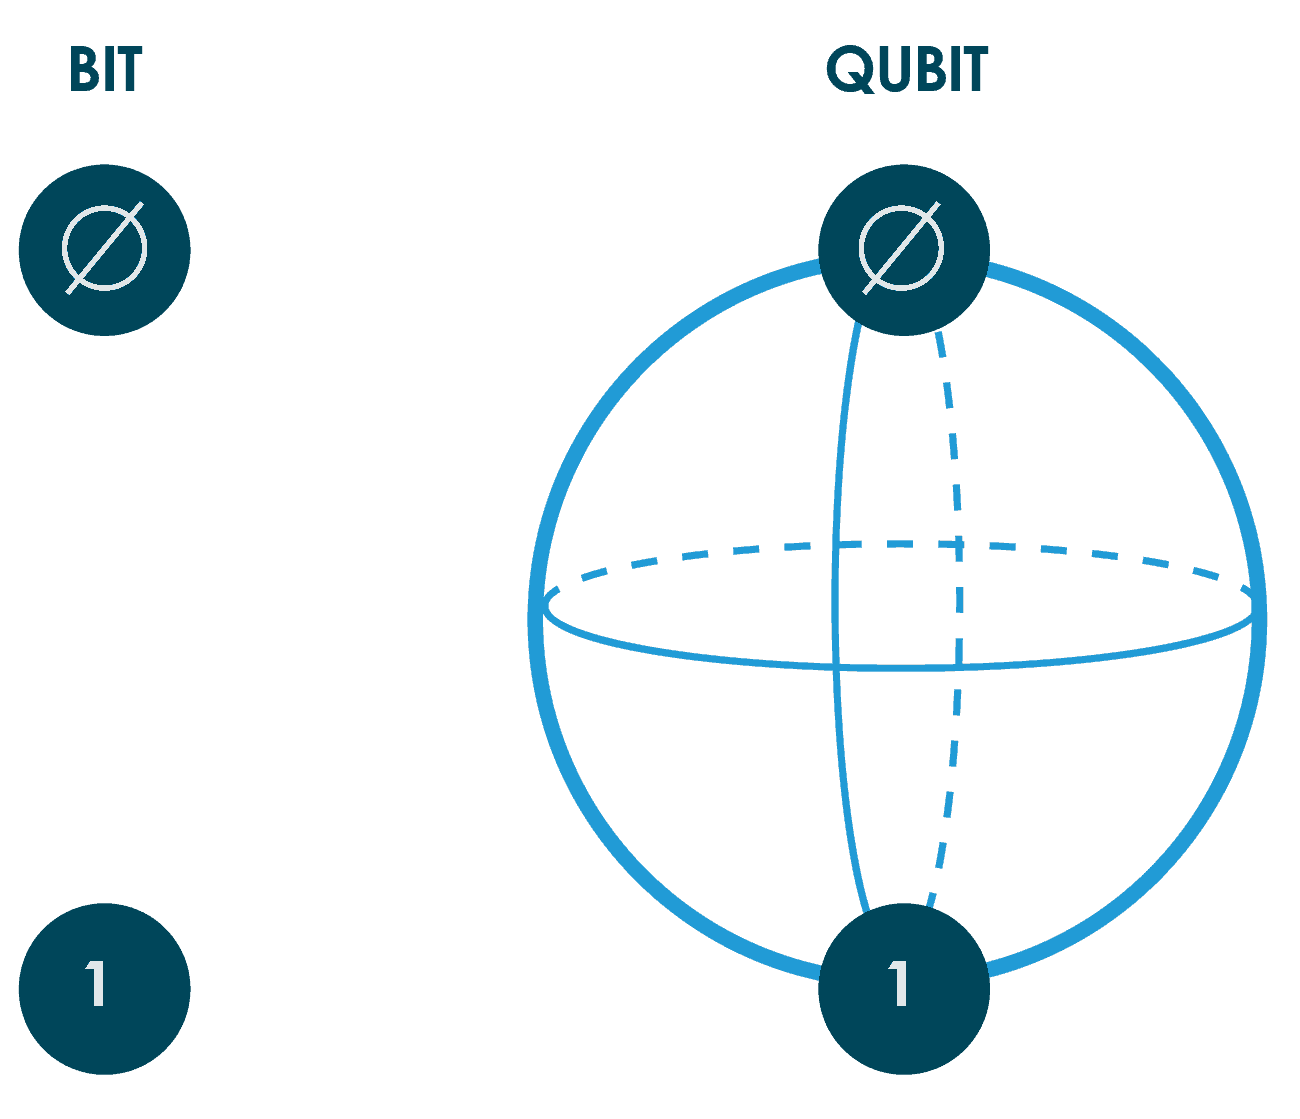
\includegraphics[width=.4\linewidth]{qubit}
        \end{figure}
    
\end{frame}

\begin{frame}{What is a qubit?}
		\begin{itemize}
			\item What does it mean to be 0 and 1 simultaneously?
			
			    It's a matter of probability during measurement
			
            \item Bra-ket qubit representation:
            \begin{columns}[T,onlytextwidth]
			\column{0.33\textwidth}
			\centering
			\begin{align*}
			    \lvert 0\rangle
			     = 
                \begin{bmatrix}
                1 \\
                0
                \end{bmatrix}
            \end{align*}
			
			\column{0.33\textwidth}
			\centering
            \begin{align*}
			    \lvert 1\rangle
			    = 
                \begin{bmatrix}
                0 \\
                1
                \end{bmatrix}
            \end{align*}
            
            \column{0.33\textwidth}
			\centering
            \begin{align*}
			    \lvert \psi\rangle
			    = 
                \begin{bmatrix}
                \psi_0 \\
                \psi_1
                \end{bmatrix}
            \end{align*}
		\end{columns}
		
		
		\item Probability measurement:
		    \begin{align*}
			    P(\lvert \psi\rangle = 0) = \lvert\psi_0\rvert^2
			\end{align*}
			\begin{align*}
			    P(\lvert \psi\rangle = 1) = \lvert\psi_1\rvert^2
            \end{align*}
		\item Probability distribution: $\langle \psi\lvert \psi \rangle = |\psi|^2 = 1 \ \forall \ \psi$

        \end{itemize}
\end{frame}

\begin{frame}{Multi-qubit system and entanglement}
    How can we represent 2 or more qubits with bra-kets? 
    
    With tensor products and longer vectors
    \begin{align*}
	    \lvert AB\rangle
		=
		\begin{bmatrix}
        a_0 \\       
        a_1 \\
        \end{bmatrix}
		\otimes
        \begin{bmatrix}
        b_0 \\       
        b_1 \\
        \end{bmatrix}
        =
        \begin{bmatrix}
        a_0 b_0 \\
        a_0 b_1 \\
        a_1 b_0 \\
        a_1 b_1 \\
        \end{bmatrix}
    \end{align*}
    By stacking $n$ qubits we can represent $2^n$ infinite precision numbers
    
    \centering
    $P(A = 0, B = 1) = \lvert a_0 b_1 \rvert^2 $
\end{frame}


\begin{frame}{Multi-qubit system and entanglement}
    How can we represent state $\lvert 00\rangle + \lvert 11\rangle $ with a tensor product? 
    
    We can't as there is no set of values for $a_0, a_1, b_0, b_1$ that allows it.
    \begin{align*}
	    \lvert AB\rangle
		=
		\begin{bmatrix}
        a_0 b_0 \\
        a_0 b_1 \\
        a_1 b_0 \\
        a_1 b_1 \\
        \end{bmatrix}
    \end{align*}
    
    However, we can still create this state with quantum circuits. The resulting state is said to be entangled as measuring one qubit immediately tells us the state of the other.
    \begin{align*}
	    \lvert 00\rangle + \lvert 11\rangle 
		=
		\begin{bmatrix}
        1/\sqrt{2} \\
        0 \\
        0 \\
        1/\sqrt{2} \\
        \end{bmatrix}
    \end{align*}
\end{frame}
